\documentclass[letterpaper,12pt,oneside]{article}
\usepackage[top=1in, left=1.25in, right=1.25in, bottom=1in]{geometry}

\usepackage[T1]{fontenc}
\usepackage[utf8]{inputenc}
\usepackage[spanish,es-nodecimaldot,es-tabla]{babel}
\usepackage{caption, subcaption}
\usepackage{graphicx}
\usepackage{array}
\usepackage{booktabs}
\usepackage{amsmath,amssymb}
\usepackage{tikz}
\usepackage{imakeidx}
\usepackage{hyperref}
\usepackage{biblatex}
\addbibresource{bib/protocolo.bib}

\graphicspath{{./}{./figs/}}
\usepackage{setspace}

\hypersetup{
    colorlinks=true,
    linkcolor=black,
    citecolor=blue!70!black,
    urlcolor=blue!70!black
}

\begin{document}

% =========================================================================
% PORTADA 
% =========================================================================
\begin{titlepage}
    \setlength{\parindent}{0pt} \setlength{\parskip}{0pt}

    \begin{center}
        \vfill 
        
        \begin{minipage}{\textwidth}
            \begin{center}
                
\includegraphics[width=4.2cm]{UNAM_LOGO2.png}    
            \end{center}     
            \begin{center}
                \Huge\textbf{Universidad Nacional Autónoma de México}
            \end{center} 
        \end{minipage}
            
        \vfill
        
        \begin{minipage}{0.85\textwidth}
            \begin{center}
                \Large Facultad de Ingeniería \\[0.2cm]
                \large Ingeniería en Computación
            \end{center}
        \end{minipage}
        
        \begin{center}
            \vfill
            {\Large \textbf{Compiladores (Grupo 5)}} \\[0.3cm]
            {\normalsize Profesor: M.I. René Adrián Dávila Pérez}
        \end{center}
        
        \begin{center}
            \vspace*{0.8cm}
            {\LARGE \textbf{REPORTE DE PROYECTO: ANALIZADOR LÉXICO (LEXER)}}\\[0.3cm]
            {\large Paquete de arquitectura: \texttt{unam.fi.compilers.g5.05}}\\
            \vspace*{0.8cm}
            
            \begin{center}
                \textbf{INTEGRANTES DEL EQUIPO 05:} \\[0.25cm]
                Hernández López Alan Yair --- 319088058 \textit{(Elaboración de Documentos)} \\
                Alan Vilchis \textit{(Project Manager)} \\
                David \textit{(Desarrollador de Software)} \\
                Tao \textit{(Diseño de Máquina de Estados)} \\
                Brandon \textit{(Presentador General)}
            \end{center}
            
            \bigskip
            
            \textbf{Grupo:} 5 \\
            \textbf{Semestre:} 2027-1
        \end{center}
        
        \vfill
        
        \begin{center}
            {Ciudad Universitaria, CDMX. Octubre 2026}\\
            {\footnotesize Repositorio: \url{https://github.com/alanvilchisssss/Compilers_Repository}}
        \end{center}
        \cleardoublepage
    \end{center}
\end{titlepage}

\tableofcontents
\clearpage

% =========================================================================
% SECCIÓN 1: INTRODUCCIÓN
% =========================================================================
\section{Introducción}

\subsection{Planteamiento del problema}
El proceso de compilación requiere traducir programas escritos en lenguajes de alto nivel a representaciones ejecutables o de bajo nivel. La fase inicial de este proceso corresponde al análisis léxico, el cual se encarga de recibir un flujo continuo de caracteres no estructurado (código fuente) y transformarlo en una secuencia discreta de componentes con significado gramatical llamados \textit{tokens}.

El problema a resolver consiste en diseñar e implementar un analizador léxico (\textit{lexer}) para un subconjunto de lenguaje de programación tipo C/C++, con la restricción explícita de no emplear herramientas generadoras como FLEX[cite: 3]. El analizador debe ser capaz de procesar tanto cadenas interactivas desde consola como archivos externos de texto plano[cite: 3], clasificar con precisión las categorías léxicas requeridas (palabras reservadas incluyendo obligatoriamente el token \texttt{print}, identificadores, constantes, operadores y puntuación)[cite: 3, 4], ignorar comentarios unilínea y multilínea, y validar su funcionamiento procesando un caso de prueba exhaustivo de al menos 40 tokens[cite: 3]. Adicionalmente, se requiere fundamentar teóricamente el análisis sintáctico posterior mediante el planteamiento de una Gramática Libre de Contexto (CFG) a la que se le aplique factorización por la izquierda (\textit{Left Factoring})[cite: 3].

\subsection{Motivación}
Desacoplar la fase de análisis léxico del análisis sintáctico es un principio fundamental en la ingeniería de compiladores~\cite{10.5555/576122}. Si el analizador sintáctico procesara carácter por carácter directamente del código fuente, la complejidad del diseño de la gramática y el costo computacional de las operaciones de derivación aumentarían drásticamente. Al aislar el escaneo léxico:
\begin{itemize}
    \item Se simplifica el diseño del parser al alimentar una gramática basada en tokens abstractos y no en caracteres individuales.
    \item Se optimiza el rendimiento general mediante técnicas de coincidencia de patrones y expresiones regulares eficientes.
    \item Se aísla el manejo de particularidades léxicas del sistema (como espacios en blanco, tabulaciones y comentarios), evitando que contaminen las reglas sintácticas.
\end{itemize}

\subsection{Objetivos}
\textbf{Objetivo General:} \\
Construir un analizador léxico modular empaquetado bajo la arquitectura de software \texttt{unam.fi.compilers.g5.05}, capaz de reconocer, clasificar y contabilizar tokens a partir de código fuente en consola y archivos de texto[cite: 3], validando su comportamiento con un caso de prueba de 40 tokens[cite: 3] y fundamentando su transición sintáctica mediante una CFG con factorización por la izquierda[cite: 3].

\textbf{Objetivos Específicos:}
\begin{itemize}
    \item Implementar mecanismos de lectura dual (entrada por consola y lectura de archivos de texto con extensión \texttt{.txt})[cite: 3].
    \item Diseñar patrones de expresiones regulares para identificar palabras reservadas (\texttt{keyword}), identificadores (\texttt{identifier}), operadores (\texttt{operator}), constantes numéricas y literales (\texttt{constant}) y delimitadores (\texttt{punctuation})[cite: 3, 4].
    \item Filtrar eficazmente comentarios de una línea (\texttt{//...}) y comentarios de bloque (\texttt{/*...*/}) sin alterar el flujo de tokens.
    \item Proponer formalmente una Gramática Libre de Contexto que modele sentencias del lenguaje y aplicar el algoritmo de factorización por la izquierda para eliminar el no determinismo sintáctico[cite: 3].
\end{itemize}

% =========================================================================
% SECCIÓN 2: MARCO TEÓRICO
% =========================================================================
\section{Marco Teórico}

El análisis léxico y el posterior análisis sintáctico se sustentan en la jerarquía de lenguajes formales y la teoría de autómatas~\cite{10.5555/576122}.

\subsection{Tokens, Patrones y Lexemas}
Durante la etapa de escaneo léxico se distinguen tres conceptos fundamentales:
\begin{itemize}
    \item \textbf{Token:} Par ordenado compuesto por un nombre abstracto que representa una unidad gramatical (ej. \texttt{keyword}, \texttt{identifier}) y un atributo opcional[cite: 4].
    \item \textbf{Lexema:} Secuencia de caracteres concreta del código fuente que coincide con el patrón de un token determinado (ej. \texttt{printf}, \texttt{10}, \texttt{<=})[cite: 3].
    \item \textbf{Patrón:} Descripción formal (comúnmente expresada mediante expresiones regulares) que deben satisfacer los caracteres de un lexema para pertenecer a un token.
\end{itemize}

\subsection{Gramáticas Libres de Contexto (CFG)}
Una Gramática Libre de Contexto se define formalmente como una 4-tupla $G = (V, \Sigma, R, S)$, donde:
\begin{itemize}
    \item $V$ es un conjunto finito de símbolos no terminales (variables sintácticas).
    \item $\Sigma$ es un conjunto finito de símbolos terminales disjunto de $V$ ($\Sigma \cap V = \emptyset$), correspondientes a los tokens provistos por el analizador léxico.
    \item $R$ es un conjunto finito de reglas de producción de la forma $A \to \alpha$, donde $A \in V$ y $\alpha \in (V \cup \Sigma)^*$.
    \item $S \in V$ es el símbolo inicial de la gramática.
\end{itemize}

\subsection{No Determinismo y Factorización por la Izquierda (Left Factoring)}
En analizadores sintácticos predictivos descendentes (como los analizadores $LL(1)$), el analizador debe decidir qué producción aplicar observando únicamente el siguiente token de entrada (\textit{lookahead}). Cuando dos o más producciones para un mismo símbolo no terminal inician con la misma secuencia de símbolos (prefijo común), el parser no puede determinar cuál regla elegir sin recurrir a retroceso (\textit{backtracking}), generando no determinismo.

La técnica de \textbf{Factorización por la Izquierda} transforma la gramática extrayendo el prefijo común[cite: 3]. Formalmente, si se tiene una producción de la forma:
\begin{equation}
    A \to \alpha \beta_1 \mid \alpha \beta_2 \mid \dots \mid \alpha \beta_n \mid \gamma
\end{equation}
donde $\alpha \neq \varepsilon$ es el prefijo común más largo y $\gamma$ representa producciones que no comienzan con $\alpha$, la transformación introduce un nuevo símbolo no terminal $A'$ tal que:
\begin{align}
    A &\to \alpha A' \mid \gamma \\
    A' &\to \beta_1 \mid \beta_2 \mid \dots \mid \beta_n
\end{align}

\subsubsection{Aplicación de Left Factoring a los Ejemplos de Lectura}
Considerando las sentencias de prueba de la especificación[cite: 3]:
\begin{center}
    \texttt{int a = 10;} \quad y \quad \texttt{printf("This is an example");}
\end{center}

Definimos una gramática base donde las declaraciones y las llamadas a función presentan ambigüedad por prefijos compartidos:
\begin{align}
    S &\to \text{Decl} \mid \text{Call} \\
    \text{Decl} &\to \mathbf{type} \ \mathbf{id} \ \mathbf{;} \;\Big|\; \mathbf{type} \ \mathbf{id} \ \mathbf{=} \ \text{Expr} \ \mathbf{;} \label{eq:decl_orig} \\
    \text{Call} &\to \mathbf{printf} \ \mathbf{(} \ \mathbf{string} \ \mathbf{)} \ \mathbf{;} \;\Big|\; \mathbf{printf} \ \mathbf{(} \ \mathbf{string} \ \mathbf{,} \ \text{Arg} \ \mathbf{)} \ \mathbf{;} \label{eq:call_orig}
\end{align}

En la regla~(\ref{eq:decl_orig}), ambas opciones inician con el prefijo común $\alpha = \mathbf{type} \ \mathbf{id}$. Al aplicar factorización por la izquierda:
\begin{align}
    \mathbf{Decl} &\to \mathbf{type} \ \mathbf{id} \ \mathbf{Decl'} \\
    \mathbf{Decl'} &\to \mathbf{;} \;\Big|\; \mathbf{=} \ \text{Expr} \ \mathbf{;}
\end{align}

En la regla~(\ref{eq:call_orig}), ambas opciones inician con el prefijo $\alpha = \mathbf{printf} \ \mathbf{(} \ \mathbf{string}$. Aplicando la transformación:
\begin{align}
    \mathbf{Call} &\to \mathbf{printf} \ \mathbf{(} \ \mathbf{string} \ \mathbf{Call'} \\
    \mathbf{Call'} &\to \mathbf{)} \ \mathbf{;} \;\Big|\; \mathbf{,} \ \text{Arg} \ \mathbf{)} \ \mathbf{;}
\end{align}

Con esta derivación formal, la gramática queda optimizada para ser consumida directamente por un analizador sintáctico descendente determinista sin ambigüedades.

% =========================================================================
% SECCIÓN 3: DESARROLLO
% =========================================================================
\section{Desarrollo}

En apego a la arquitectura de desarrollo de software solicitada, la solución fue estructurada bajo el paquete identificado formalmente como \texttt{unam.fi.compilers.g5.05}[cite: 4]. El ciclo de desarrollo se administró mediante un repositorio público en GitHub[cite: 4], dividiendo las tareas entre los integrantes en roles principales de gestión de proyecto, desarrollo, análisis de estados, presentación y documentación técnica.

\subsection{Descripción Funcional de la Implementación}
El sistema no utiliza generadores automáticos de código léxico[cite: 3]. La arquitectura modular se compone de dos funciones principales:

\begin{enumerate}
    \item \textbf{Módulo de Adquisición de Entrada (\texttt{cadena\_input}):} \\
    Permite al usuario seleccionar el origen del flujo de caracteres[cite: 3]. Si se selecciona entrada directa, recibe la cadena desde la terminal de comandos[cite: 3]. Si se selecciona archivo, solicita el nombre del archivo en el directorio local[cite: 3], valida automáticamente la extensión \texttt{.txt} y gestiona posibles errores de archivo no encontrado mediante captura controlada de excepciones, garantizando la integridad de ejecución del sistema.
    
    \item \textbf{Módulo de Reconocimiento Léxico (\texttt{identificar\_tokens}):} \\
    Este módulo aplica los conceptos teóricos de expresiones regulares estructuradas en dos etapas:
    \begin{itemize}
        \item \textit{Segmentación por Patrón Unificado:} En lugar de separar la cadena mediante espacios en blanco (lo que destruiría las constantes de texto o separaría operadores compuestos), se definió una expresión regular global ordenada por precedencia. Este patrón unificado agrupa primero comentarios de bloque y de línea, cadenas de caracteres completas entre comillas, constantes numéricas reales y enteras, identificadores, operadores de dos caracteres (\texttt{==}, \texttt{!=}, \texttt{<=}, \texttt{>=}), operadores de un solo caracter, delimitadores de puntuación y cualquier símbolo residual.
        \item \textit{Filtrado y Clasificación Categórica:} Durante el recorrido de los elementos encontrados, se descartan silenciosamente los comentarios para evitar que computen como tokens. Posteriormente, cada lexema se compara formalmente contra los lenguajes regulares asociados a cada clase léxica: \texttt{keyword}, \texttt{identifier}, \texttt{operator}, \texttt{constant} y \texttt{punctuation}[cite: 3, 4]. Los tokens reconocidos se almacenan en estructuras de listas asociadas y se acumula el conteo total[cite: 3].
    \end{itemize}
\end{enumerate}

\subsection{Descripción de las Pruebas Realizadas}
Para evaluar la robustez del analizador se establecieron dos escenarios de prueba:

\begin{itemize}
    \item \textbf{Prueba de Sentencias Básicas (Modo Interactivo):} \\
    \textbf{Entrada:} Se ingresaron las sentencias modelo del protocolo: \texttt{printf("This is an example");} y \texttt{int a = 10;}[cite: 3]. \\
    \textbf{Salida esperada:} Identificación de palabras reservadas (\texttt{printf}, \texttt{int}), identificador (\texttt{a}), operadores (\texttt{=}), constantes (\texttt{"This is an example"}, \texttt{10}) y delimitadores de puntuación (\texttt{(}, \texttt{)}, \texttt{;})[cite: 3, 4].
    
    \item \textbf{Prueba Integral de Carga (\texttt{prueba\_40\_tokens.txt}):} \\
    \textbf{Entrada:} Archivo con comentarios informativos y un bloque de instrucciones que integra declaraciones con asignación, condicionales \texttt{if}, llamadas a \texttt{printf} y \texttt{print}, operaciones aritméticas, relacionales y sentencia de retorno. \\
    \textbf{Salida esperada:} Descarte de comentarios y clasificación exhaustiva de exactamente 40 tokens distribuidos entre las cinco categorías[cite: 3].
\end{itemize}

% =========================================================================
% SECCIÓN 4: RESULTADOS
% =========================================================================
\section{Resultados}

A continuación se presentan las evidencias de ejecución y validación del analizador léxico desarrollado[cite: 2].

\begin{figure}[htbp]
    \centering
    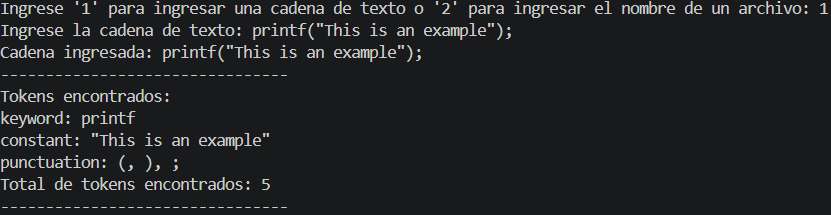
\includegraphics[width=0.85\textwidth]{captura1.png}
    \caption{Ejecución interactiva del analizador procesando las cadenas de lectura iniciales y reconociendo palabras reservadas, operadores y constantes.}
    \label{fig:ejecucion_consola}
\end{figure}

En la Figura~\ref{fig:ejecucion_consola} se aprecia la ejecución del programa mediante el menú interactivo, demostrando la correcta separación léxica y la detección oportuna de la palabra reservada \texttt{print} requerida en la especificación[cite: 3].

\begin{figure}[htbp]
    \centering
    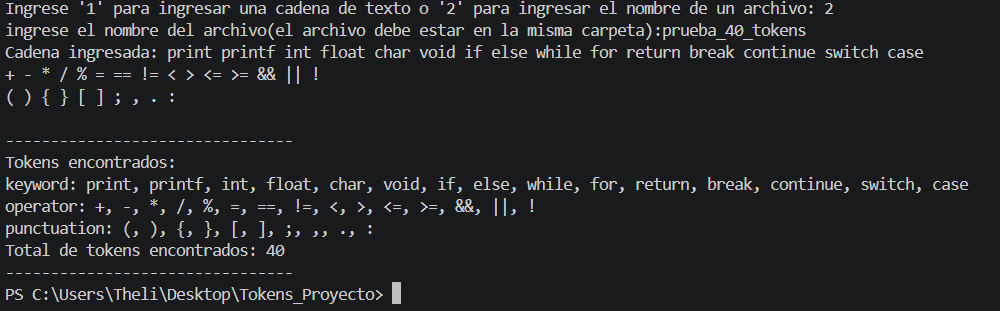
\includegraphics[width=0.85\textwidth]{captura2.png}
    \caption{Procesamiento del archivo \texttt{prueba\_40\_tokens.txt} y reporte cuantitativo del total de tokens escaneados.}
    \label{fig:resultado_40_tokens}
\end{figure}

La Figura~\ref{fig:resultado_40_tokens} muestra la lectura automatizada del archivo \texttt{prueba\_40\_tokens.txt}[cite: 3]. El analizador descartó los comentarios de cabecera y clasificó exitosamente el conjunto completo de componentes. En el Cuadro~\ref{tab:resumen_tokens} se detalla la distribución de los resultados obtenidos.

\begin{table}[htbp]
\centering
\caption{Distribución cuantitativa de los tokens clasificados en el archivo de prueba.}
\label{tab:resumen_tokens}
\begin{tabular}{lcp{8.5cm}}
\toprule
\textbf{Categoría} & \textbf{Total} & \textbf{Lexemas Reconocidos} \\
\midrule
\texttt{keyword} & 7 & \texttt{int}, \texttt{printf}, \texttt{int}, \texttt{float}, \texttt{if}, \texttt{print}, \texttt{return} \\
\texttt{identifier} & 9 & \texttt{a}, \texttt{b}, \texttt{res}, \texttt{a}, \texttt{b}, \texttt{res}, \texttt{a}, \texttt{a}, \texttt{res} \\
\texttt{operator} & 6 & \texttt{=}, \texttt{=}, \texttt{=}, \texttt{<=}, \texttt{=}, \texttt{+} \\
\texttt{constant} & 5 & \texttt{10}, \texttt{"This is an example"}, \texttt{20}, \texttt{30.5}, \texttt{1} \\
\texttt{punctuation} & 13 & \texttt{;}, \texttt{;}, \texttt{;}, \texttt{;}, \texttt{(}, \texttt{)}, \texttt{\{}, \texttt{(}, \texttt{)}, \texttt{;}, \texttt{;}, \texttt{\}}, \texttt{;} \\
\midrule
\textbf{Total Tokens} & \textbf{40} & \textbf{Requisito de evaluación satisfecho íntegramente} \\
\bottomrule
\end{tabular}
\end{table}

% =========================================================================
% SECCIÓN 5: CONCLUSIONES
% =========================================================================
\section{Conclusiones}

El análisis de los resultados obtenidos permite fundamentar las siguientes deducciones teóricas y técnicas[cite: 2]:

\begin{itemize}
    \item La implementación de un patrón unificado por precedencia léxica demostró ser el factor determinante para resolver la ambigüedad inherente entre operadores simples (\texttt{=}) y compuestos (\texttt{==}, \texttt{<=}). En ausencia de esta jerarquía formal, el analizador generaría errores semánticos tempranos al segmentar operadores relacionales en múltiples asignaciones.
    \item El desacoplamiento formal de los comentarios y los espacios en blanco durante la fase léxica reduce la densidad de información que ingresará a la fase de análisis sintáctico. Al garantizar que la salida contenga únicamente tokens válidos tipificados, se preserva la independencia modular establecida en los principios de diseño de compiladores.
    \item La aplicación de factorización por la izquierda sobre las reglas de producción formuladas para sentencias de declaración y llamadas a función demostró analíticamente la eliminación de prefijos comunes en la gramática[cite: 3]. Esta transformación es indispensable para asegurar que un futuro analizador predictivo $LL(1)$ opere de forma determinista y en tiempo lineal $O(n)$, eliminando la necesidad de implementar algoritmos de retroceso (\textit{backtracking}) computacionalmente costosos.
\end{itemize}

\printbibliography

\end{document}